\myChapter{une approche orientée attributs pour le contrôle d'accès basé sur la hiérarchie organisationnelle (AHOr-BAC)}{}\label{chapAHOr-BAC}

\myMiniToc{section}{Sommaire} 

\mySection{Concepts de base du modèle AHOr-BAC}{}\label{sectionConcept}

\mySubSection{Organisation}{}\label{sectionOrganisation} 
Une organisation est un ensemble d'individus, regroupés au sein d'une structure régulée, ayant un système de communication pour faciliter la circulation de l'information, dans le but de répondre à des besoins et d'atteindre des objectifs déterminés. Elle est représenté dans notre modèle par l'entité \textit{Organisation}

\mySubSection{Employé Métier}{}\label{sectionEmployeMetier} 
Il représente une personne physiquement identifiable ayant un rôle actif dans l'organisation. C'est la seule entité réellement active dans l'organisation. Tout comme dans HOr-BAC, ce concept permet d'empêcher la création des entités virtuelles dans le système d'information par le super-utilisateur. Car, si l'utilisateur est une personne physique, il pourra être facilement contrôlé. les employé métier peuvent avoir un ou plusieurs attributs, et chaque attribut peut avoir une ou plusieurs valeurs d'attributs qui sont représentés par les entités \textit{AttributE} et \textit{valeurAttributE} respectivement. Dans notre modèle, on attribut une ou plusieurs valeurs d'attributs d'employés à chaque Employé métier. Ce qui est représenté par la relation suivante: %\textit{Useruavassignment} \subseteq \textit{Users} \times \textit{Userattributevalues}

\begin{figure}[h!]
    \centering
		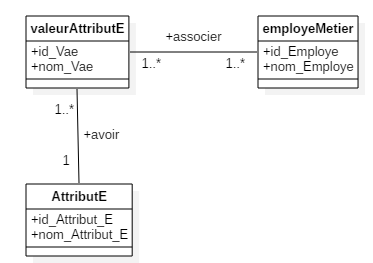
\includegraphics[scale=0.7]{chap3/images/employe_attribut.png}
    \caption{Affectation des valeurs d'attribut d'employé aux employé métiers}
	 \label{figemploye}
\end{figure} 

\mySubSection{Ressource}{}\label{sectionRessource}

l'entité \textit{ressource} est utilisée pour organiser l'ensemble des données et informations de l'organisation et exprime les entités passives du système. Par exemple, le dossier médical d'un patient, les dossiers d'inscription. les ressources peuvent avoir un ou plusieurs attributs, et chaque attribut peut avoir une ou plusieurs valeurs d'attributs de ressource qui sont représentés par les entités \textit{AttributR} et \textit{valeurAttributR} respectivement. Notre modèle, attribue une ou plusieurs valeurs d'attribut de ressource à chaque ressource. cela est matérialisé par la relation suivante:

\begin{figure}[h!]
    \centering
		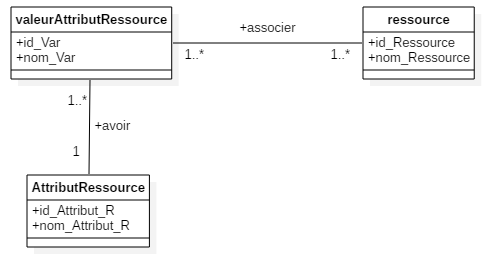
\includegraphics[scale=0.7]{chap3/images/ressource_attribut.png}
    \caption{Affectation des valeurs d'attribut de ressource aux ressources}
	 \label{figressource}
\end{figure} 

\mySubSection{Requête}{}\label{sectionRequête}

Tout comme HOr-BAC, une requête est définie dans notre modèle comme une demande fait par un employé métier dans  le système. Une requête doit avoir les informations suivantes: le nom de l'émetteur, la ressource, l'action et le nom su destinataire. Il existe deux type de requêtes à savoir :\\
- la requête à exécution indirecte (différée): il s'agit ici, d'une requête qui nécessite automatiquement la validation du supérieur hiérarchique de l'employé qui initié la requête.\\
- la requête à exécution indirecte (réelle): il s'agit ici, d'une requête qui n'a pas besoin d'être traité par le supérieur hiérarchique de l'employé qui émet la requête. 

\mySubSection{Unité organisationnelle et hiérarchie organisationnelle}{}\label{sectionUnitéOrg}

Dans HOr-BAC, une unité organisationnelle est définie comme étant le regroupement des unités administratives et opérationnelles. Ce qui implique qu'une unité organisationnelle peut jouer soit un rôle administrative soit un rôle opérationnel.
\mySubSubSection{Unité opérationnelle}{}\label{sectionUnitéOpérationnelle}
Elle représente l'ensemble des employés métiers ayant les mêmes formations, les mêmes rôles et une fonction spécifique dans une organisation. Elle ne prend aucune décision sur le fonctionnement de l'organisation et ne fait qu'obéit aux décisions qui lui ont été données par l'unité administrative qui la subordonne. Exemple : comptabilité, enseignant. 
\mySubSubSection{Unité administrative}{}\label{sectionUnitéAdministrative}
Elle représente l'ensemble des unités décisionnelles de l'organisation. Cette entité permet de représenter les fonctions de contrôle, de supervision, et de validation des requêtes émises dans le SI. Elle peut être placée sur une unité opérationnelle ou sur une autre unité administrative. Exemple : département, rectorat et décanat dans une université.
\paragraph{}Grâce à la structure organisationnelle d'une organisation, il est possible de dégager l'ordre hiérarchique entre deux unités organisationnelle.

\mySubSection{Structure organisationnelle}{}\label{sectionStructureOrg}

La structure organisationnelle est définie comme étant la représentation schématique des liens hiérarchiques et fonctionnels d'une entreprise ou d'une organisation. Elle permet de préciser les niveaux de responsabilités et le mode de communication interne à l'organisation. Pour pouvoir contrôler les différentes opérations des utilisateurs du système d'information dans une organisation, nous allons ressortir la structure organisationnelle hiérarchique de cette dernière.
\paragraph{} En effet, nous représentons cette structure hiérarchique par un arbre comportant les nœuds et les feuilles signifiant respectivement les unités administratives et les unités opérationnelles de l'organisation. Une unité opérationnelle se représente sous la forme UO1,P où 1 représente le premier niveau et p représente la p-ième unité opérationnelle. Par ailleurs, une unité administrative est représentée sous la forme UAn,p où n est le niveau hiérarchique et p la p-ième unité administrative. La figure 2.10 présente une structure organisationnelle à 5 niveaux hiérarchiques.

\begin{figure}[h!]
    \centering
		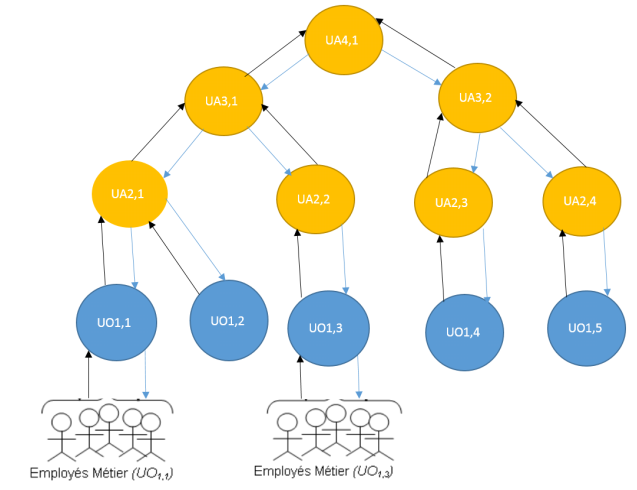
\includegraphics[scale=0.7]{chap3/images/structureorg.png}
    \caption{Structure organisationnelle d'une organisation}
	 \label{figstructure}
\end{figure} 

\mySubSection{Contexte}{}\label{sectionContexte}

Dans notre modèle, le \textit{contexte} définie une situation ou des circonstances dans lesquelles les organisations accordent des permissions à des rôles pour réaliser des requêtes sur des vues. Il est indépendant des employés métiers et des ressources. Tout comme l'employé métier et la ressource, un contexte peut avoir un ou plusieurs attributs. ces attributs permettent d'exprimer des contraintes relatives aux unités organisationnelles, aux ressources, et aux employés métiers. Chaque attribut peut avoir une ou plusieurs valeurs d'attribut de contexte qui sont représentés par les entités \textit{AttributC} et \textit{valeurAttributC} respectivement. Dans notre modèle, on associe une ou plusieurs valeurs d'attribut de contexte à chaque contexte. Ce qui est capturé par la relation suivante:

\begin{figure}[h!]
    \centering
		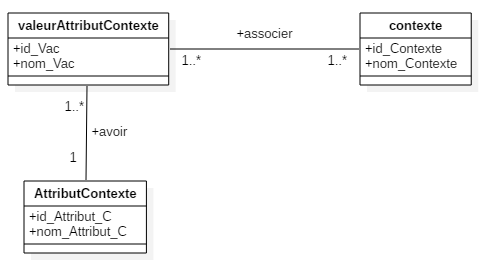
\includegraphics[scale=0.7]{chap3/images/contexte_Attribut.png}
    \caption{Affectation des valeurs d'attributs de contexte aux contextes}
	 \label{figcontexte}
\end{figure} 

\mySubSection{Mode de traitement}{}\label{sectionModeTraitement}

Tout comme dans HOr-BAC, l'entité \textit{Mode de traitement} dans notre modèle permet de matérialiser l'état d'urgence de traitement d'une requête. En effet, le changement d'état ressource doit être faite après validation ou non du supérieur hiérarchique de l'employé qui a émit la requête demandant accès à cette ressource.

\mySubSection{Règles}{}\label{sectionRègle}

Afin de permettre le contrôle des politiques de sécurité en fonction des attributs, nous introduisons dans notre modèle l'entité \textit{Règle}. Une règle permet d'activer ou de déactiver les permissions de bas niveau. C'est-à-dire liées aux actions concrètes que réalise les employés métiers sur des ressources. 
\paragraph{} Dans AHOr-BAC, les règles qui restreignent la disponibilité des permissions pour les employés métiers peuvent être composées des valeurs d'attributs d'employé, des valeurs d'attribut de contexte et/ou des valeurs d'attribut de ressource.

\mySection{Présentation des relations dans AHOr-BAC}{}\label{sectionRelation} 

\mySubSection{Employé métier et Unité opérationnelle}{}\label{sectionEmployeUniteO}

La relation \textit{Emploie} permet de matérialiser le fait qu'une organisation emploie un employé métier dans une unité opérationnelle.Cette relation est représentée à la figure \ref{figemploie}.

\begin{figure}[h!]
    \centering
		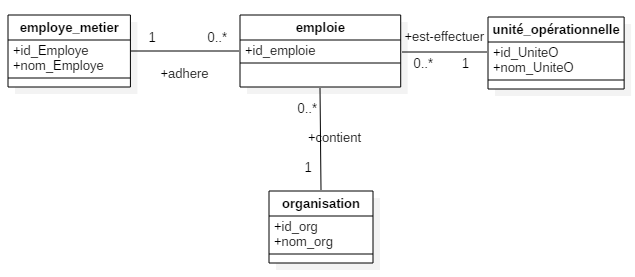
\includegraphics[scale=0.7]{chap3/images/emploie.png}
    \caption{Diagramme de classes de la relation emploie}
	 \label{figemploie}
\end{figure} 

\mySubSection{Employé métier et Unité Administrative}{}\label{sectionEmployeUniteA}

La relation \textit{Nomme} permet de matérialiser le fait que dans une organisation une unité administrative est dirigée par un employé métier. Cette relation est représentée à la figure \ref{fignomme}.

\begin{figure}[h!]
    \centering
		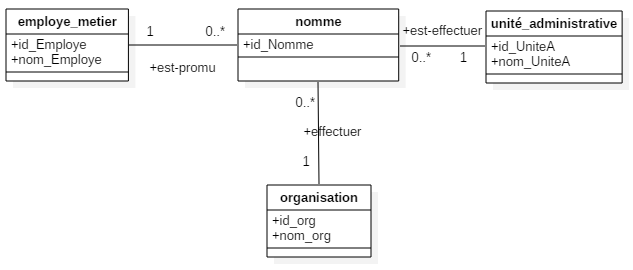
\includegraphics[scale=0.7]{chap3/images/nomme.png}
    \caption{Diagramme de classes de la relation nomme}
	 \label{fignomme}
\end{figure} 

\mySubSection{Unité Administrative et Unité Opérationnelle}{}\label{sectionUnitéOUniteA}

La relation \textit{Place-sous} représente le fait que dans une organisation les rôles opérationnels sont subordonnés aux rôles administratifs. Car l'unité opérationnelle a une fonction d'exécution, alors que l'unité administrative a une fonction de contrôle.

\begin{figure}[h!]
    \centering
		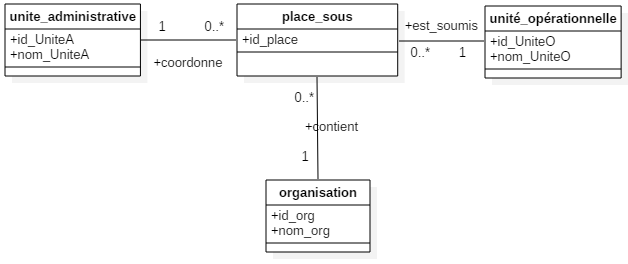
\includegraphics[scale=0.7]{chap3/images/place-sous.png}
    \caption{Diagramme de classes de la relation place-sous}
	 \label{figplace-sous}
\end{figure} 

\mySubSection{Unité Administrative et Unité Administrative}{}\label{sectionUnitéAUniteA}

La relation entre les unité administratives est matérialiser dans  notre modèle par la relation \textit{Subordonne}. En effet, dans la hiérarchie De l'organisation, en dehors du conseil d'administration qui est une unité spéciale, toutes les unités administratives sont  subordonnées à une autre qui assure le contrôle de ses activités. Pour cette relation il ne peut y avoir dans une organisation une unité administrative subordonnée à elle-même. Cette relation est représentée à la figure \ref{figsubordonne}.

\begin{figure}[h!]
    \centering
		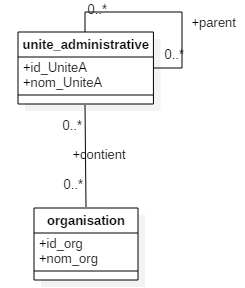
\includegraphics[scale=0.7]{chap3/images/subordonne.png}
    \caption{Diagramme de classes de la relation subordonne}
	 \label{figsubordonne}
\end{figure} 

\mySubSection{Les ressources et les vues}{}\label{sectionRessourceetVue}

La relation entre les unité administratives est matérialiser dans  notre modèle par la relation \textit{Utilise}. En effet, une même ressource peut être considérée de différentes manières dans une organisation en fonction des unités organisationnelles à partir desquelles cette ressource est vue. Une vue est un regroupement de ressources sur lesquelles on applique les mêmes politiques de sécurité. Suivant les organisations une même vue peut être définir différemment. Ainsi utilise permet de matérialiser le fait qu'une organisation utilise une ressource dans une vue.

\begin{figure}[h!]
    \centering
		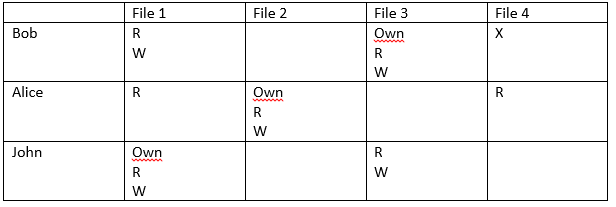
\includegraphics[scale=0.7]{chap2/images/ACM.png}
    \caption{Diagramme de classes de la relation Utilise}
	 \label{figAcm}
\end{figure} 

\mySubSection{Les actions et les requêtes}{}\label{sectionActionRequêtes}

La relation entre les unité administratives est matérialiser dans  notre modèle par la relation \textit{Considère}. En effet, les politiques de sécurité spécifient les accès aux ressources par les unités organisationnelles et régulent les actions opérées sur le système. Dans notre modèle, l'entité Action englobe principalement les actions informatiques comme "lire", "écrire", "envoyer". Et l'entité Requête englobe principalement les demandes comme "consulter", "modifier", "transmettre", "ajouter", "supprimer". Considère permet de représenter le fait qu'une  organisation considère une action comme faisant partie d'une requête.

\begin{figure}[h!]
    \centering
		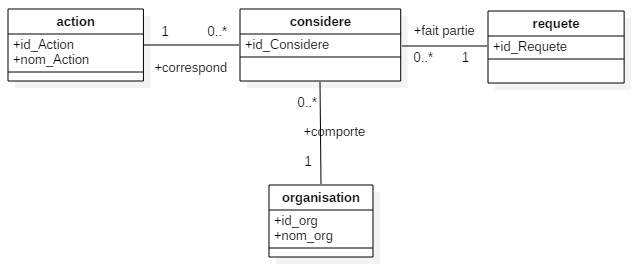
\includegraphics[scale=0.7]{chap3/images/considere.png}
    \caption{Diagramme de classes de la relation considère}
	 \label{figconsidere}
\end{figure} 

\mySubSection{La relation définit}{}\label{sectionDéfinit}

 La relation \textit{définit} permet de vérifier si un employé métier a le droit d'appliquer une requête sur une ressource et dans un contexte prédéfinie par l'organisation. Cette relation est représentée à la figure \ref{figdefini}.

\begin{figure}[h!]
    \centering
		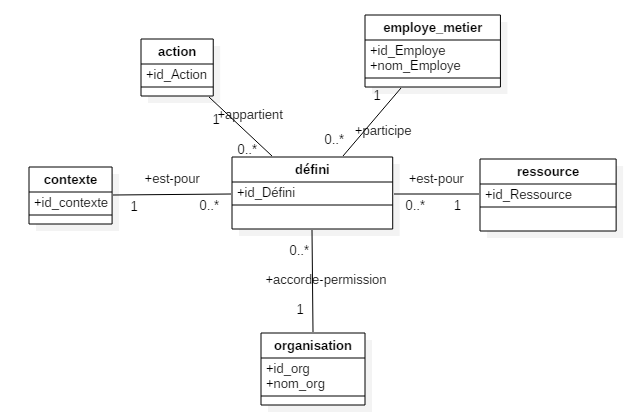
\includegraphics[scale=0.7]{chap3/images/defini.png}
    \caption{Diagramme de classes de la relation définit}
	 \label{figdefini}
\end{figure} 

\mySubSection{Permissions}{}\label{sectionPermission}

Une permission matérialise le fait qu'une organisation autorise une unité organisationnelle de traiter ou d'émettre une requête donnée dans une vue donnée selon un contexte précis et un mode de traitement bien définie. De ce fait, nous distinguons deux types de permissions qui sont:\\
- les permissions dites de préparation: encore appelées permissions opérationnelles. Elles permettent aux unités opérationnelles de préparer (initier, émettre ou soumettre.) des requêtes à leurs hiérarchie. Elles sont matérialisées par la relation permission-opérationnelle qui relie les entités organisation, unité opérationnelle, requête, vue, contexte et mode de traitement. Cette relation est représentée à la figure \ref{figpermissionO}.\\
- les permissions dites de validation: encore appelées permissions administratives, elles permettent aux unités administratives de traiter (contrôler, rejeter, valider et/ou transmettre) les requêtes  provenant dans unités opérationnelles. Elles sont matérialisées par la relation permission-administrative qui permet de relier les entités organisation, unité opérationnelle, unité administrative, requête, vue, contexte et mode de traitement. Cette relation est représentée à la figure \ref{figpermissionA};

\begin{figure}[h!]
    \centering
		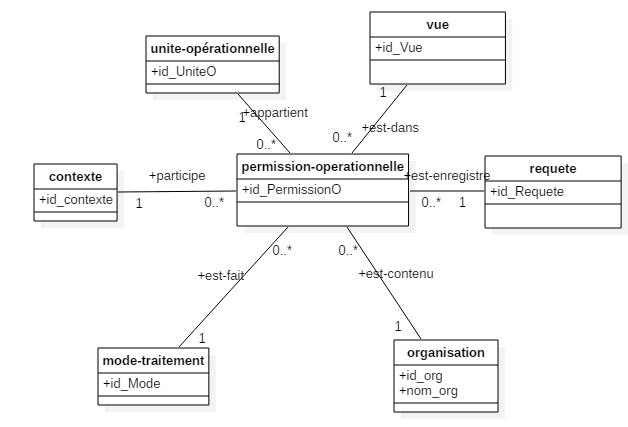
\includegraphics[scale=0.7]{chap3/images/permissionO.png}
    \caption{Diagramme de classes de la relation permission-opérationnelle}
	 \label{figpermissionO}
\end{figure} 

\begin{figure}[h!]
    \centering
		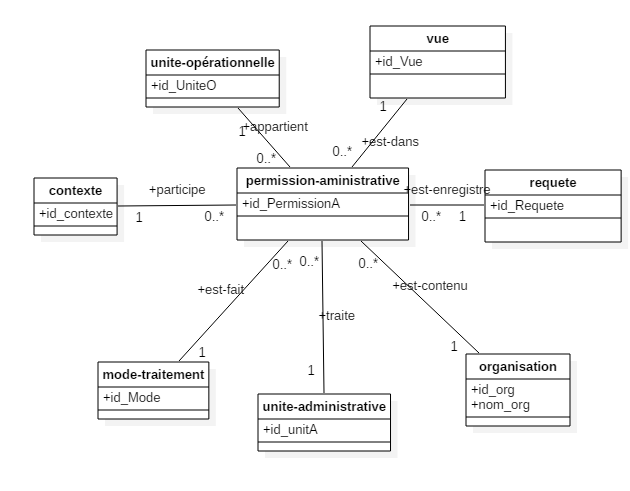
\includegraphics[scale=0.7]{chap3/images/permissionA.png}
    \caption{Diagramme de classes de la relation permission-Administrative}
	 \label{figpermissionA}
\end{figure} 

\mySubSection{Les relations peut-suggérer et peut-traiter}{}\label{sectionSuggererTraiter}

Les permissions vues plus haut ne permettent qu'à une organisation donnée de spécifier les permissions accordées aux unités organisationnelles suivant un contexte précis. Mais ne permettent pas de décrire des actions concrètes que réalisent les employés sur les ressources. Ainsi nous avons implémentés le concept de contrôle d'accès de bas niveau à travers les relations suivantes : \\
- \textit{Peut-suggérer} : cette relation permet à un employé d'obtenir la permission de suggérer l'application d'une action sur une ressource donnée. Cette relation est représentée à la figure \ref{figpeut-suggerer}.\\
- \textit{Peut-traiter} : cette relation matérialise le fait que le supérieur hiérarchique d'un employé a l'autorisation de traiter les suggestions d'application d'une action donnée sur une ressource donnée. Cette relation est représentée à la figure \ref{figpeut-traiter}.

\begin{figure}[h!]
    \centering
		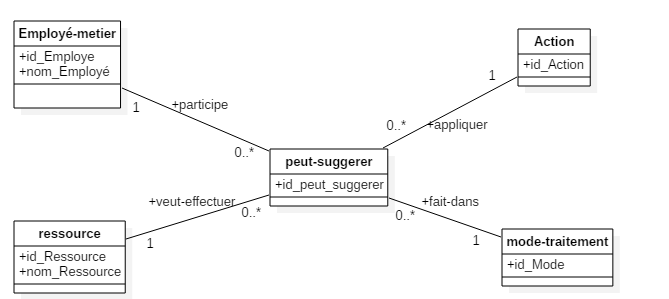
\includegraphics[scale=0.7]{chap3/images/peut-suggerer.png}
    \caption{Diagramme de classes de la relation peut-suggérer}
	 \label{figpeut-suggerer}
\end{figure} 

\begin{figure}[h!]
    \centering
		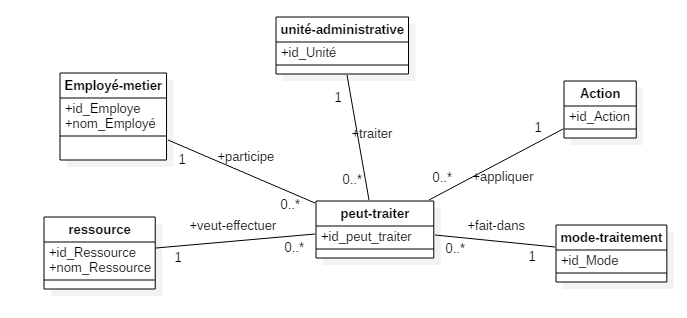
\includegraphics[scale=0.7]{chap3/images/peut-traiter.png}
    \caption{Diagramme de classes de la relation peut-traiter}
	 \label{figpeut-traiter}
\end{figure} 
%\mySubSection{Attribution des règles aux unités organisationnelles}{}\label{sectionAttributionRegleUnité}

%Dans notre modèle, une règle peut être assignée à plusieurs  unités organisationnelles, et une unité organisationnelle peut avoir plusieurs règles. Cette façon de faire permet de réduire l'espaces des règles applicables pour une unité organisationnelle, de minimiser le temps d'évolution de la disponibilité des unités organisationnelles pour un employé. Ainsi notre approche peut restreindre les unités organisationnelles.

\mySubSection{Attribution des Règles aux Permissions de bas niveau}{}\label{sectionAttributionReglePermission}

Dans notre modèle, une règle peut être assignée à plusieurs permissions, et une permission peut avoir plusieurs règles. Le Fait que, notre modèle, associe directement un ensemble de règles basées sur les attributs aux permissions permet de réduire l'espaces des règles applicables pour une permission, de minimiser le temps d'évolution de la disponibilité des permissions pour un  employé métier. Car au lieu  d'évaluer directement une autorisation on évolue l'ensemble des règles applicables pour cette autorisation et s'il y a une règle vraie alors la permission est accordée à l'employé.  Ainsi notre approche peut restreindre les permissions. 

\begin{figure}[h!]
    \centering
		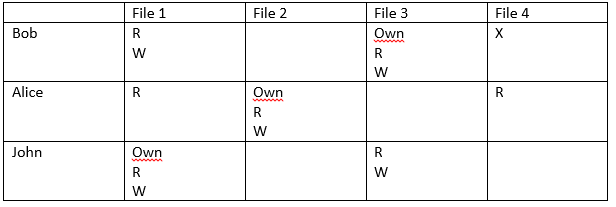
\includegraphics[scale=0.7]{chap2/images/ACM.png}
    \caption{Affectation des règles aux permissions de bas niveaux 1}
	 \label{figAcm}
\end{figure} 

\begin{figure}[h!]
    \centering
		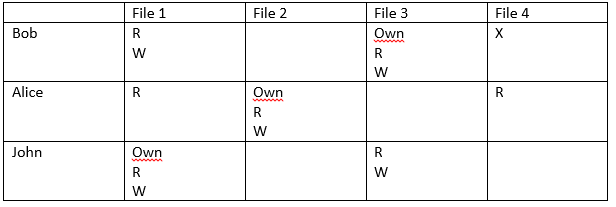
\includegraphics[scale=0.7]{chap2/images/ACM.png}
    \caption{Affectation des règles aux permissions de bas niveaux 2}
	 \label{figAcm}
\end{figure} 
\mySection{Algorithme du parapheur électronique}{}\label{sectionParapheur}

Tout comme HOr-BAC, nous introduisons dans notre modèle la notion de parapheur électronique. Il s'agit d'un processus de traitement automatique sécurisé basé sur le modèle HOr-BAC. Il consiste à supposer que la quasi-totalité des actions dans une organisation se fait sur la demande et chaque demande obtient une validation pour une exécution effective dans le système sinon, la demande est rejetée. Ce processus est mis en œuvres en trois phases.

\mySubSection{La phase d'initialisation du parapheur électronique}{}\label{sectionPhaseInitialisation}

Cette phase permet la création des différentes entités du modèle HOr-BAC y compris les différentes relations qui existent entre elles. Elle est réalisée à travers six processus que sont :

\myDescription{\textit{Créer-org}}{Cette procédure crée la structure organisationnelle dans un
arbre et retourne la racine qui est la plus grande unité administrative de l'organisation ;}

\myDescription{\textit{Créer-emp}}{Cette procédure prend la liste du personnel et affecte chacun à une unité organisationnelle en utilisant la relation \textit{Emploie} et \textit{Nomme};}

\myDescription{\textit{Créer-vue}}{Elle prend la liste des ressources et crée les différentes vues de l'organisation, en utilisant la relation \textit{Utilise} ;}

\myDescription{\textit{Créer-requête}}{Elle prend la liste des actions et crée les différentes requêtes de l'organisation, en utilisant la relation \textit{Considère} ;}

\myDescription{\textit{Créer-mode-traitement}}{Cette procédure crée les différents modes de traitement utilisés dans l'organisation ;}

\myDescription{\textit{Créer-permission}}{Elle associe à chaque unité organisationnelle les Permissions
opérationnelles ou les Permissions administratives suivant les cas, et donne les permissions opérationnelles aux employés métier et nomme les administrateurs;}

\paragraph{} Contrairement à HOr-BAC, dans notre modèle nous définissons à ce niveau un nouveau processus qui nous permettra d'associer un ensemble de règles basées sur les attributs afin de permettre un contrôle de bas niveau et à grain fin des ressources.
  
%\myDescription{\textit{Créer-règle-unité-organisationnelle}}{Elle associe à chaque unité organisation un ensemble de règles en utilisant la relation \textit{attribuer} }

\myDescription{\textit{Créer-règle-permission-bas-niveau}}{Elle associe à chaque permission de bas niveau un ensemble de règles en utilisant la relation \textit{attribuer} }

\mySubSection{La phase d'émission d'une requête du parapheur électronique}{}\label{sectionPhaseEmission}


Cette phase est déclenché lorsqu'un employé qui veut effectuer une action sur une ressource protégée du système émet par le biais de son unité opérationnelle une requête demandant l'accès à une vue du système. Tout comme dans HOr-BAC, cette phase du parapheur électronique, dans notre modèle permet d'effectuer un contrôle de bas niveau des ressources auxquelles on souhaite y accéder. C'est-à-dire qu'on aimerait savoir si un employé métier peut oui ou non effectuer une action sur une ressource ou tout simplement signaler à son supérieur hiérarchique qu'il aimerait effectuer une action données sur les ressources protégées du système. La particularité de notre modèle réside dans le fait que, cette phase ne se base pas simplement sur les permissions opérationnelles pour accorder l'accès aux ressources du système, mais aussi sur des règles qui permettent un contrôle à grain fin des ressources. Ces règles comme nous l'avons spécifier plus haut sont une combinaison des valeurs d'attribut d'employé métier, des valeurs d'attribut de ressource et/ou des valeurs d'attribut de contexte. 

\paragraph{} Cette phase est capturée par un algorithme qui prend en entrée l'employé métier qui émet une requête, la requête, l'action, la vue, le contexte,le mode de traitement de la requête et un fichier contenant l'ensemble des règles d'accès. Lors de l'émission d'une requête, notre algorithme se charge de vérifier l'identité de l'émetteur de la requête. Après confirmation de l'identité de ce dernier, notre algorithme récupère l'unité opérationnelle qui émet la requête, vérifie si cette unité à une permission opérationnelle qui lui permet de réaliser la requête sur une vue donnée dans un contexte précis et selon un mode de traite de la requête défini. Si l'unité opérationnelle ne possède pas de permission alors l'accès à la ressource est refusé. Sinon, on récupère l'employé et on vérifie s'il est employé dans cette unité opérationnelle par l'organisation; si oui, on récupère la ressource de la demande dans la politique de sécurité et vérifie si celle-ci est utilisée comme vue dans l'organisation. Si cette vérification n'est pas correcte, la requête n'aboutit pas ; sinon ce processus récupère l'action de la demande dans la table action et contrôle si elle est considérée comme la requête q au sein de l'organisation. Dans le cas où il y a échec du contrôle, la demande est non valide ; dans le cas contraire, le processus continue ses vérifications en récupérant le contexte de la demande dans la politique de sécurité située dans la base de données de l'organisation et vérifie si l'émetteur a la permission de proposer une application de l'action a sur la ressource r dans le contexte c au sein de l'organisation. La demande échoue si celui-ci n'a pas cette permission et le processus d'émission continu ses vérifications. Si cette permission
lui est définie, l'algorithme récupère le fichier XML qui contient les règles basée sur les attributs d'employé métier, de ressource et de contexte qui est stocké dans la base de donnée et vérifie si au plus une règle permet d'activer la permission qui donne le droit à l'employé d'effectuer une action donnée sur une ressource. Si aucune règle n'est remplit, la demande est annulée. Sinon l'algorithme récupère le mode de traitement dans la base de données. A cet effet, il existe deux modes de traitement d'une requête à savoir : les modes de traitement temps réel et temps diffère.\\
— Lorsque le mode de traitement est temps réel, la demande de l'émetteur n'est pas contrôlée par une unité administrative. Par conséquent le processus d'émission du parapheur électronique enregistre cette requête dans la base de données de l'organisation. Ainsi la requête préalablement émise par l'émetteur est finalement validée.\\
— Lorsque le mode de traitement est temps différé, la demande émise par l'émetteur doit être automatiquement validée par au moins une unité administrative de la structure organisationnelle. Alors le processus donne la possibilité à l'employé de faire une suggestion à son supérieur hiérarchique. puis la requête sera sauvegardée dans la base de donnée et une alerte sera envoyée a l'un des supérieur hiérarchique de ce dernier.

\begin{figure}[h!]
    \centering
		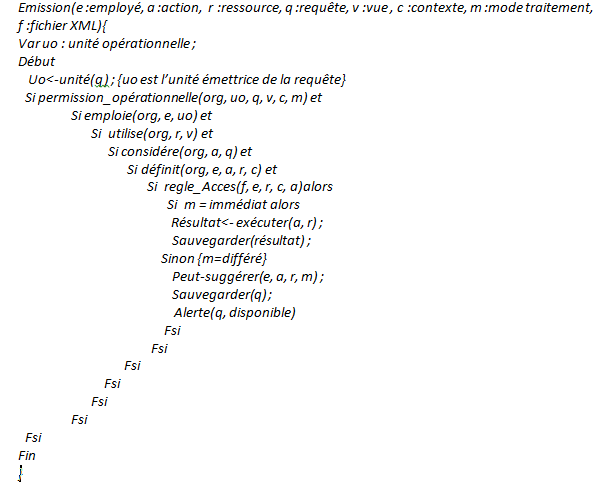
\includegraphics[scale=0.7]{chap3/images/emission.png}
    \caption{Algorithme d'émission du parapheur électronique}
	 \label{figemission}
\end{figure} 

\mySubSection{La phase de traitement d'une requête du parapheur électronique}{}\label{sectionPhasetraitement}

Cette phase est déclenché lorsque le supérieur hiérarchique d'un employé métier reçoit une alerte du système lui indiquant qu'une requête vient d'être soumis par ce dernier et qu'elle attend d'être traiter par lui afin d'accorder ou pas l'accès aux ressources protégées du système. Tout comme dans HOr-BAC, cette phase du parapheur électronique, dans notre modèle permet d'effectuer un contrôle de bas niveau des ressources auxquelles on souhaite y accéder. C'est-à-dire qu'on aimerait savoir si le supérieur hiérarchique d'un employé peut ou ne peut pas autoriser à ce dernier d'effectuer une action sur une ressource ou tout simplement transmettre cette requête à une autorité au dessus de la sienne pour qu'elle valide ou refuse l'exécution de la requête par l'employé. La particularité de notre modèle réside dans le fait que, cette phase ne se base pas simplement sur les permissions administratives pour accorder l'accès aux ressources du système, mais aussi sur des règles basées sur des attributs qui permettent un contrôle à grain fin des ressources. 

\paragraph{} Cette phase est capturée par un algorithme qui prend en entrée l'employé métier qui est chargé de traiter la requête, la requête, l'action, la vue, le contexte,le mode de traitement de la requête et un fichier contenant l'ensemble des règles d'accès. Lors du traitement d'une requête, notre algorithme se charge de vérifier l'identité de l'employé qui est chargé du traitement de la requête. Après confirmation de l'identité de ce dernier, notre algorithme récupère tout d'abord l'unité administrative de cet employé puis l'unité opérationnelle qui émet la requête, et vérifie si cette unité à une permission administrative qui lui permet d'autoriser à l'unité organisationnelle de l'employé qui à émit la requête de réaliser la requête sur une vue donnée dans un contexte précis et selon un mode de traite de la requête défini. Si l'unité administrative ne possède pas de permission alors la demande est rejetée. Sinon, le processus de vérification peut continuer. Alors on récupère le supérieur hiérarchique chargé du traitement de la requête et l'émetteur de la requête et on vérifie si dans l'organisation ce dernier est le chef de l'employé qui a émit la requête. Si tel n'est pas le cas, il y a échec de la requête; sinon le processus vérifie si l'employé (supérieur hiérarchique) est nommé en tant qu'une unité administrative dans l'organisation. Dès que cette vérification est invalide, il y a échec de la requête ; dans le cas contraire, ce processus continue son exécution en récupérant la ressource de la requête dans la base de données et contrôle si cette ressource est utilisée comme vue au sein de l'organisation ; si tel est le cas, le processus récupère l'action dans la base de données et teste si cette dernière est considérée comme la requête dans l'organisation. Si tel n'est pas le cas la demande échoue.

\paragraph{} Dans le cas contraire, il récupère le contexte de l'unité administrative autorisée à valider la requête dans la table contexte et vérifie si dans cette organisation, cette unité est autorisée à valider la requête demandant d'effectuer l'action a sur la ressource r, dans le contexte émise par l'émetteur de la requête. Si c'est le cas, l'algorithme récupère le fichier XML qui contient les règles basée sur les attributs d'employé métier, de ressource et de contexte qui est stocké dans la base de donnée et vérifie si au plus une règle permet d'activer la permission qui donne le droit à l'employé de validé ou de refusé l'exécution de la requête. Si aucune règle n'est remplit, la demande est annulée. Dans le cas contraire, il teste si la hauteur du destinataire de la requête ou la hauteur du supérieur hiérarchique qui traite la demande est égale à la profondeur de l'émetteur de la requête et vérifie si le mode de traitement du supérieur hiérarchique est en temps réel, la vérification étant correcte, ce dernier donne son avis qui peut être une validation ou un refus. Dans le cas où il y a acceptation, le processus effectue l'action demandée sur la ressource dans la base de données. Dans le cas où cet avis est un refus, il y a échec de la demande. Si son mode de traitement est temps différé, le processus recherche le prochain supérieur hiérarchique qui doit donner son accord sur la demande et recommence son exécution.

\begin{figure}[h!]
    \centering
		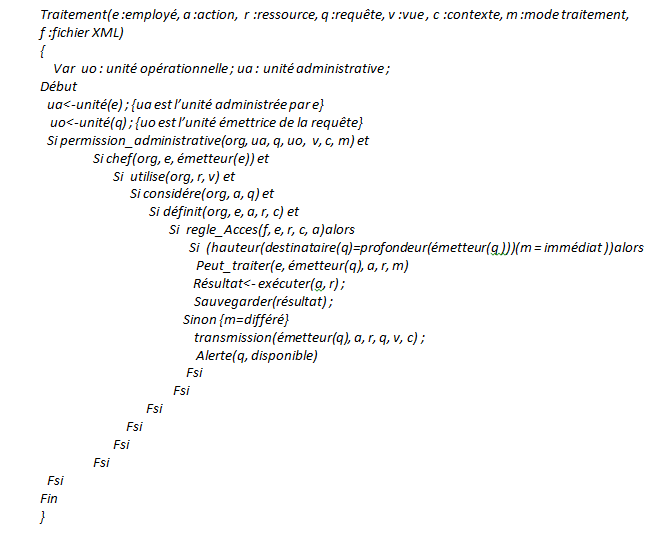
\includegraphics[scale=0.7]{chap3/images/traitement.png}
    \caption{Algorithme de traitement du parapheur électronique}
	 \label{figtraitement}
\end{figure} 

\mySubSection{Étude de cas: spécification d'une politique de sécurité avec AHOr-BAC}{}\label{sectionExemple}

Dans cette section, nous montrerons comment spécifier des règles en utilisant les attributs de diverses entités et discuterons également de la façon dont leur association avec des permissions peut assurer la disponibilité fine-grainée des objets pour les utilisateurs.

%\begin{table}
	%\caption{Un tableau}
	%\begin{flushleft}
	%\begin{tabular}[t]{lcp{5.3cm}l}
	%$\langle A,w_{1} \rangle$ & $\longrightarrow$ & $(P_{1}, [\langle C,u \rangle, \langle B,v \rangle])%$ & si $w_{1}=u[v]$ \\
	
	%\end{tabular}
	%\begin{tabular}[t]{lcp{5.3cm}l}
	
	%$\langle A,w_{2} \rangle$ & $\longrightarrow$ & $(P_{1}, [\langle C,u \rangle, \langle B,w_{11}    \rangle])$ & si $w_{2}=uw_{11}$ avec $w_{11}=[_{\omega}\, ]_{\omega}$ \\
	
	%\end{tabular}
	%\begin{tabular}[t]{lcp{5.3cm}l}
	
	%$\langle A,w_{3} \rangle$ & $\longrightarrow$ & $(P_{2}, [\,])$ & si $w_{3}=\epsilon$\\
	
	%\end{tabular}
	%\begin{tabular}[t]{lcp{5.3cm}l}
	
	%$\langle A,w_{4} \rangle$ & $\longrightarrow$ & $(A_{\omega}, [\,])$ & si $w_{4}=(_{\omega}\, )_{\omega}$\\
	
	%\end{tabular}
	%\begin{tabular}[t]{lcp{5.3cm}l}
	
	%$\langle B,w_{5} \rangle$ & $\longrightarrow$ & $(P_{3}, [\langle C,u \rangle, \langle A,v \rangle])$ & si $w_{5}=u(v)$ \\
	
	%\end{tabular}
	%\begin{tabular}[t]{lcp{5.3cm}l}
	
	%$\langle B,w_{6} \rangle$ & $\longrightarrow$ & $(P_{3}, [\langle C,u \rangle, \langle A,w_{4} \rangle])$ & si $w_{6}=uw_{4}$ \\
	
	%\end{tabular}
	%\begin{tabular}[t]{lcp{5.3cm}l}
	
	%$\langle B,w_{7} \rangle$ & $\longrightarrow$ & $(P_{4}, [\langle B,u \rangle, \langle B,v \rangle])$ & si $w_{7}=[u][v]$\\
	
	%\end{tabular}
	%\begin{tabular}[t]{lcp{5.3cm}l}
	
	%$\langle B,w_{8} \rangle$ & $\longrightarrow$ & $(P_{4}, [\langle B,w_{11} \rangle, \langle B,v \rangle])$ & si $w_{8}=w_{11}[v]$\\
	
	%\end{tabular}
	%\begin{tabular}[t]{lcp{5.3cm}l}
	
	%$\langle B,w_{9} \rangle$ & $\longrightarrow$ & $(P_{4}, [\langle B,u \rangle, \langle B,w_{11} \rangle])$ & si $w_{9}=[u]w_{11}$\\
	
	%\end{tabular}
	%\begin{tabular}[t]{lcp{5.3cm}l}
	
	%$\langle B,w_{10} \rangle$ & $\longrightarrow$ & $(P_{4}, [\langle B,w_{11} \rangle, \langle B,w_{11} \rangle])$ & si $w_{10}=w_{11}w_{11}$\\
	
	%\end{tabular}
	%\begin{tabular}[t]{lcp{5.3cm}l}
	
	%$\langle B,w_{11} \rangle$ & $\longrightarrow$ & $(B_{\omega}, [\,])$ & si $w_{11}=[_{\omega}\, ]_{\omega}$\\
	
	%\end{tabular}
	%\begin{tabular}[t]{lcp{5.3cm}l}
	
	%$\langle C,w_{12} \rangle$ & $\longrightarrow$ & $(P_{5}, [\langle A,u \rangle, \langle C,v \rangle])%$ & si $w_{12}=(u)v$ \\
	
	%\end{tabular}
	%\begin{tabular}[t]{lcp{5.3cm}l}
	
	%$\langle C,w_{13} \rangle$ & $\longrightarrow$ & $(P_{5}, [\langle A,w_{4} \rangle, \langle C,v \rangle])$ & si $w_{13}=w_{4}v$ \\
	
	%\end{tabular}
	%\begin{tabular}[t]{lcp{5.3cm}l}
	
	%$\langle C,w_{14} \rangle$ & $\longrightarrow$ & $(P_{6}, [\langle C,u \rangle, \langle C,v \rangle])%$ & si $w_{14}=uv\neq\epsilon$\\
	
	%\end{tabular}
	%\begin{tabular}[t]{lcp{5.3cm}l}
	
	%$\langle C,w_{15} \rangle$ & $\longrightarrow$ & $(C_\omega,[\,])$ & si $w_{15}=\epsilon$\\
	
	%\end{tabular}
	%\end{flushleft}
%\end{table}
